
The testing described in Section \ref{sec:randerr} describes the process of
evaluating the methodology with test cases drawn from the training database.
It is also helpful to test the methodology against real assays of \gls{SNF}.
The \gls{SFCOMPO} database was created to allow access to these sorts of
measurements linked to the reactor operation parameters being predicted in this
work. \cite{sfcompo}. The only parameter not part of the \gls{SFCOMPO} database
is the time since irradiation, so that is not predicted here. 

\begin{figure}[!htb]
    \centering
    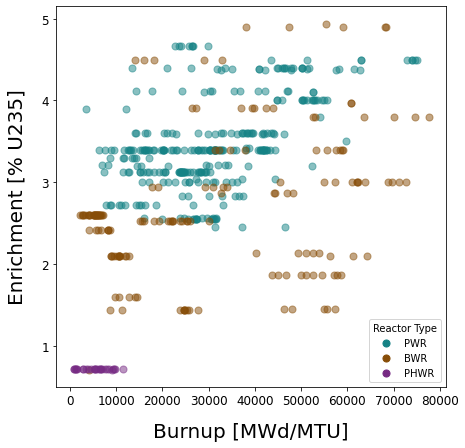
\includegraphics[width=0.7\textwidth]{./chapters/exp1/sfcompo_scatter_viz.png}
    \caption{Scatter plot showing the range of reactor operation parameters in 
             the \gls{SFCOMPO} testing set that are being predicted.}
    \label{fig:sfcoscatter}
    \todo[inline]{increase tick size, maybe show comparison against training 
                  E v B scatter plot}
\end{figure}

There are 505 test cases that are able to be compared against the training
database.  The number of each reactor type is as follows: 312 \gls{PWR}s, 165
\gls{BWR}s, and 28 \gls{PHWR}s. The space of enrichment and burnup values is
visualized in Figure \ref{fig:sfcoscatter}. These are sufficienty represented
in the training set design, as pictured in Figure \ref{fig:trainhist}.

\begin{table}[!ht]
  \centering
  \begin{tabular}{|>{\raggedleft}m{0.6in}
                                 m{0.4in}
                  |>{\raggedleft}m{0.6in}
                                 m{0.4in}
                  |>{\raggedleft}m{0.6in}
                                 m{0.4in}|}
    \toprule
    am241  & 237 & nd145 & 162 & sm147 & 97  \\
    am242m & 110 & nd146 & 139 & sm149 & 97  \\
    am243  & 203 & nd148 & 275 & sm150 & 97  \\
    cm242  & 214 & nd150 & 121 & sm151 & 97  \\
    cm244  & 269 & np237 & 155 & sm152 & 97  \\
    cs134  & 113 & pu238 & 369 & u234  & 355 \\
    cs137  & 185 & pu239 & 505 & u235  & 479 \\
    eu154  & 100 & pu240 & 505 & u236  & 462 \\
    nd143  & 162 & pu241 & 504 & u238  & 433 \\
    nd144  & 113 & pu242 & 505 &       &     \\ \bottomrule
  \end{tabular}
  \caption{.}
  \todo[inline]{fix up formatting}
  \label{tbl:missing}
\end{table}

There is one main issue with using this as a testing set: missing nuclide
measurements.  The feature set of 29 nuclides in Table \ref{tbl:nucmass} was
chosen based on the frequency of these measurements being present in
\gls{SFCOMPO} at an arbitrary level of 100 measurements. This happened before
filtering, so there are some nuclide measurements present at under 100 counts.
Each nuclide's frequency in \gls{SFCOMPO} is listed in Table \ref{tbl:missing}.



\begin{table}[!ht]
  \centering
  \begin{tabular}{@{}l|lll|lll@{}}
  \toprule
                   & \multicolumn{3}{l|}{Accuracy Scores} & \multicolumn{3}{l}{Balanced Accuracy Scores} \\ \toprule
  Null Handling    & kNN        & DTree      & MLL       & kNN           & DTree         & MLL           \\ \midrule
  Imputed Nulls    & 0.52       & 0.60       & 0.39      & 0.09          & 0.12          & 0.00          \\
  Zero-value Nulls & 0.45       & 0.42       & 0.72      & 0.21          & 0.30          & 0.63          \\ \bottomrule
  \end{tabular}
  \caption{sfcompo reactor accuracies.}
  \label{tbl:sfcorxtr}
\end{table}

\begin{figure}[!ht]
    \centering
    \begin{subfigure}[b]{0.49\textwidth}
        \centering
        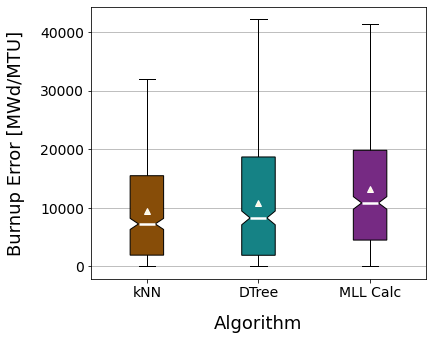
\includegraphics[width=\textwidth]{./chapters/exp1/sfcompo_boxplots_impnull_burn.png}
        \caption[]{Caption.}
        %\label{fig:}
    \end{subfigure}
    \hfill
    \begin{subfigure}[b]{0.49\textwidth}
        \centering
        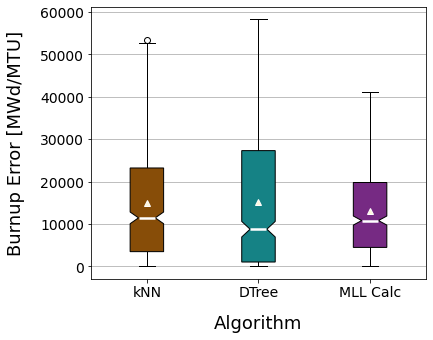
\includegraphics[width=\textwidth]{./chapters/exp1/sfcompo_boxplots_0null_burn.png}
        \caption[]{Caption.}
        %\label{fig:}
    \end{subfigure}
    \caption{sfcompo burnup boxplots.}
    \label{fig:sfcoburn}
\end{figure}

\begin{table}[!ht]
  \centering
  \begin{tabular}{@{}l|lll|lll@{}}
  \toprule
                   & \multicolumn{3}{l|}{Mean Errors [GWd/MTU]} & \multicolumn{3}{l}{Median Errors [GWd/MTU]} \\ \toprule
  Null Handling    & kNN           & DTree         & MLL           & kNN            & DTree          & MLL    \\ \midrule
  Imputed Nulls    & 9.43          & 10.89         & 13.17         & 7.26           & 8.28           & 10.84  \\
  Zero-value Nulls & 14.88         & 15.18         & 3.53          & 11.47          & 8.79           & 1.70   \\ \bottomrule
  \end{tabular}
  \caption{sfcompo burnup errors.}
  \label{tbl:sfcoburn}
\end{table}

\begin{figure}[!ht]
    \centering
    \begin{subfigure}[b]{0.49\textwidth}
        \centering
        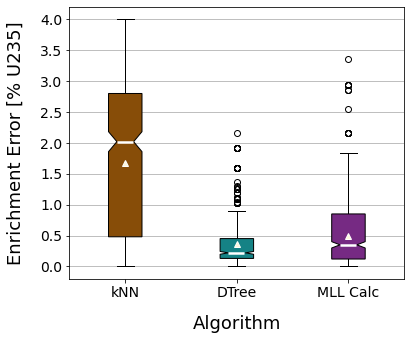
\includegraphics[width=\textwidth]{./chapters/exp1/sfcompo_boxplots_0null_enri.png}
        \caption[]{Caption.}
        %\label{fig:}
    \end{subfigure}
    \hfill
    \begin{subfigure}[b]{0.49\textwidth}
        \centering
        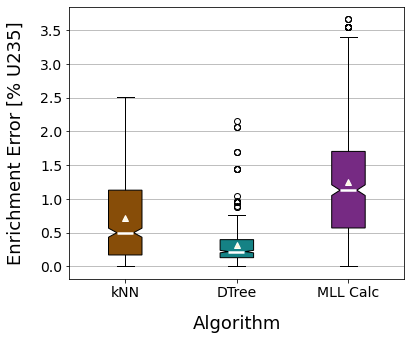
\includegraphics[width=\textwidth]{./chapters/exp1/sfcompo_boxplots_impnull_enri.png}
        \caption[]{Caption.}
        %\label{fig:}
    \end{subfigure}
    \caption{sfcompo enrichment boxplots.}
    \label{fig:sfcoenri}
\end{figure}

\begin{table}[!ht]
  \centering
  \begin{tabular}{@{}l|lll|lll@{}}
  \toprule
                   & \multicolumn{3}{l|}{Mean Errors [\% U235]} & \multicolumn{3}{l}{Median Errors [\% U235]} \\ \toprule
  Null Handling    & kNN           & DTree          & MLL          & kNN            & DTree          & MLL    \\ \midrule
  Imputed Nulls    & 0.72          & 0.31           & 1.25         & 0.50           & 0.22           & 1.13   \\
  Zero-value Nulls & 1.67          & 0.36           & 0.49         & 2.02           & 0.22           & 0.35   \\ \bottomrule
  \end{tabular}
  \caption{sfcompo enrichment errors.}
  \label{tbl:sfcoenri}
\end{table}

